\documentclass{beamer}
\setbeamercovered{transparent}

\usepackage{epstopdf}
\usepackage[inline]{asymptote}

\mode<presentation> %?

\usetheme{Frankfurt}
\usepackage{helvet}
\usepackage{mathptmx}
%\usefonttheme{professionalfonts}
\usefonttheme[onlymath]{serif}
\usefonttheme{structurebold}

%\renewcommand{\familydefault}{Futura}
%\setsansfont{Verdana}

\setlength{\unitlength}{\paperwidth}

% width, height, title, content
\newcommand{\SizedBlock}[4]{
  \begin{block}{#3}
    \parbox[t][#2\paperwidth][t]{#1\paperwidth}{#4}    
  \end{block}
}

% w1, c1, w2, c2
\newcommand{\TwoColumns}[4]{
  \vspace{-0.02\paperwidth}
  \begin{columns}[t]
    \begin{column}{#1\paperwidth}
      #2
    \end{column}\hspace{-0.02\paperwidth}
    \begin{column}{#3\paperwidth}
      #4
    \end{column}
  \end{columns}
}

% w1, c1, w2, c2, w3, c3
\newcommand{\ThreeColumns}[6]{
  \vspace{-0.02\paperwidth}
  \begin{columns}[t]
    \begin{column}{#1\paperwidth}
      #2
    \end{column}\hspace{-0.07\paperwidth}
    \begin{column}{#3\paperwidth}
      #4
    \end{column}\hspace{-0.07\paperwidth}
	\begin{column}{#5\paperwidth}
      #6
    \end{column}
  \end{columns}
}

% height, title1, content1, title2, content2
\newcommand{\TwoColumnBlocksW}[6]{
  \TwoColumns{
        #6}{
        \SizedBlock{#6}{#1}{#2}{#3}}{
        #6}{
        \SizedBlock{#6}{#1}{#4}{#5}}
}

% height, title1, content1, title2, content2
\newcommand{\TwoColumnBlocks}[5]{
  \TwoColumnBlocksW{#1}{#2}{#3}{#4}{#5}{0.4}
}

% height, title1, content1, title2, content2, title3, content3
\newcommand{\ThreeColumnBlocks}[7]{
  \ThreeColumns{
        0.24}{
        \SizedBlock{0.24}{#1}{#2}{#3}}{
        0.24}{
        \SizedBlock{0.24}{#1}{#4}{#5}}{
        0.24}{
        \SizedBlock{0.24}{#1}{#6}{#7}}
}

\newcommand{\PutPic}[3]{
  \put(#1){\includegraphics[#2\paperwidth]{./img/#3}}
}

\usepackage{color}

\begin{document}
\title{General Planar Quadrilateral Mesh Design Using Conjugate Direction Field \\ \textcolor{yellow}{[YangLiu SigAsia11]}}
\author{Tengfei Jiang}

\newcommand{\FPP}[2]{\frac{\partial #1}{\partial #2}}
\begin{frame}
  \titlepage
\end{frame}

\section{Outline}
\begin{frame}{Outline}
\begin{itemize}
  \item Notation
  \item Motivation
  \item Details
    \begin{itemize}
    \item Conjugate Direction Field(CDF) Generation
      \begin{itemize}
      \item Smoothness measurement
      \item Feature Preserving
      \end{itemize}
    \item CDF Editing
    \item Planar Meshing Generation
    \end{itemize}
  \item Results
  \item Conclusion
\end{itemize}
\end{frame}

\section{Details}
\begin{frame}{Notation}
\begin{block}{Cross Field}
\begin{figure}[!htb]
  \includegraphics[height=0.8in]{./img/cross-field.png}
  \includegraphics[height=0.8in]{./img/4-sys.png}
\end{figure}
\end{block}
\begin{block}{Conjugate Direction Field}
\TwoColumns{0.3}{
\begin{figure}
\centering
\includegraphics[height=1.0in]{./img/cdf.png}
\end{figure}
}{0.55}{

$V_p$ and $W_p$ are conjugate, iff $\prod_p (v_p,w_p)=0$.

In $R^3$, the condition is written as:
\[\kappa_1(v_i,e_1)(w_i,e_1)+\kappa_2(v_i,e_2)(w_i,e_2)=0\]
}
\end{block}
\end{frame}

\begin{frame}{Motivation}
\begin{itemize}
\item In quadrilateral meshing, cross field plays an important role. While complex feature preserving requirements make it hard for orthogonal frame field to fulfill it.
\begin{figure}[!htb]
\includegraphics[height=1.0in]{./img/f1.png}
\end{figure}
\item Planar quadrilateral mesh is the conjugate curve network.
%which is defined to be two families of one-parameter curves that cover a smooth surface, and their tangent vectors v,w at an arbitrary point x on a surface are con- jugate
\end{itemize}
\end{frame}

\subsection{CDF Smoothness}
\begin{frame}{Requirements of direction field}
\invisible{\begin{itemize}
\item As smooth as possible
\item Satisfy users' direction constraint
\item Satisfy users' topology constraint
\end{itemize}}
\end{frame}


\begin{frame}{Requirements of direction field}
\begin{itemize}
\item As smooth as possible
\item Satisfy users' direction constraint
\item Satisfy users' topology constraint
\end{itemize}
\end{frame}

\begin{frame}{Smooth Measurement}
Q: How to define the difference between $(v_i,w_i),(v_j,w_j)$?
\invisible{
\begin{figure}[!htb]
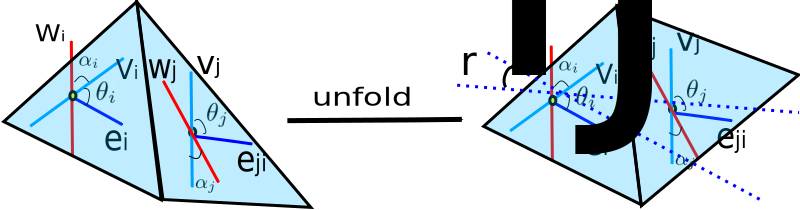
\includegraphics[height=1.0in]{./img/twoframe-unfold.png}
\end{figure}
\begin{eqnarray*}
C_1(e_{ij}) &=& \theta_j + q\alpha_j + r_{ij}-\theta_i+p_1\pi\\
C_2(e_{ij}) &=& \theta_j + (1-q)\alpha_j + r_{ij}-(\theta_i+\alpha_i)+p_2\pi
\end{eqnarray*}
where $q\in\{0,1\}$, and $p_1,p_2\in Z$
}
\end{frame}


\begin{frame}{Smooth Measurement}
\textcolor{red}{Q: How to define the difference between $(v_i,w_i),(v_j,w_j)$?}
\begin{figure}[!htb]
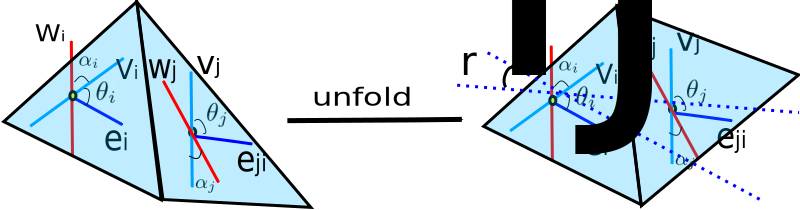
\includegraphics[height=1.0in]{./img/twoframe-unfold.png}
\end{figure}
\begin{eqnarray*}
C_1(e_{ij}) &=& \theta_j + q\alpha_j + r_{ij}-\theta_i+p_1\pi\\
C_2(e_{ij}) &=& \theta_j + (1-q)\alpha_j + r_{ij}-(\theta_i+\alpha_i)+p_2\pi
\end{eqnarray*}
where $q\in\{0,1\}$, and $p_1,p_2\in Z$
\end{frame}

\begin{frame}{Smooth Measurement}
Q: How to smooth the difference?\smallskip

\invisible{
A: $\left\{\begin{array}{cc}
C_1(e_{ij})|_{q=0}&=0\\
C_2(e_{ij})|_{q=0}&=0
\end{array}
\right.$ 
or 
$\left\{\begin{array}{cc}
C_1(e_{ij})|_{q=1}&=0\\
C_2(e_{ij})|_{q=1}&=0
\end{array}
\right.$}
\end{frame}

\begin{frame}{Smooth Measurement}
Q: How to smooth the difference?\smallskip

A: $\left\{\begin{array}{cc}
C_1(e_{ij})|_{q=0}&=0\\
C_2(e_{ij})|_{q=0}&=0
\end{array}
\right.$ 
or 
$\left\{\begin{array}{cc}
C_1(e_{ij})|_{q=1}&=0\\
C_2(e_{ij})|_{q=1}&=0
\end{array}
\right.$
\end{frame}

\begin{frame}{Smooth Measurement}
Q: How to smooth the difference?\smallskip

A: $\left\{\begin{array}{cc}
C_1(e_{ij})|_{q=0}&=0\\
C_2(e_{ij})|_{q=0}&=0
\end{array}
\right.$ 
or 
$\left\{\begin{array}{cc}
C_1(e_{ij})|_{q=1}&=0\\
C_2(e_{ij})|_{q=1}&=0
\end{array}
\right.$ 
\textcolor{red}{Hard to optimize!}
\end{frame}

\begin{frame}{Smooth Measurement}
\begin{figure}[!htb]
\includegraphics[height=1.0in]{./img/P.png}
\caption{$P_1,P_2$}
\end{figure}
$(v_i|w_i)P=(v_j|w_j)$. $P$ is a signed-permutation matrix, if $(v_i|w_i)$ and $(v_j|w_j)$ are smooth.

$P_1=\left(\begin{array}{cc}
0 & 1\\
-1 & 0
 \end{array}  \right)$ $P_2=\left(\begin{array}{cc}
-1 & 0\\
0 & -1
 \end{array}  \right)$
\end{frame}

\begin{frame}{Smooth Measurement}
\begin{figure}[!htb]
\includegraphics[height=1.0in]{./img/P.png}
\caption{$P_1,P_2$}
\end{figure}
$(v_i|w_i)P=(v_j|w_j)$. $P$ is a signed-permutation matrix, if $(v_i|w_i)$ and $(v_j|w_j)$ are smooth.

\textcolor{red}{Smooth Measurement$:=$ Diff(P, signed-permutation matrix)}
\end{frame}

\begin{frame}{Smooth Measurement}
\begin{block}{Signed Permutation matrix}
$P_{ij}$ is a signed permutation matrix iff two conditions hold: $P_{ij}^{-1} = P_{ij}^T$ and $\frac{C_1(e_1{ij})+C_2(e_2{ij})}{2}=0$
\end{block}
$E_s=\|D\|^2+\|E\|^2$, $D$ is about the first term and $E$ is the second one.
\end{frame}

\begin{frame}{User Control}
\begin{block}{Feature Preserving}
\begin{figure}[!htb]
\includegraphics[height=0.8in]{./img/feature.png}\hspace{1.0in}
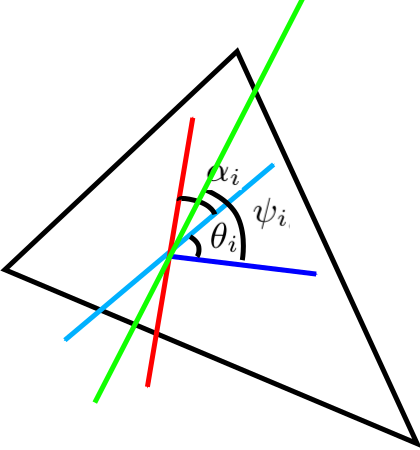
\includegraphics[height=0.8in]{./img/feature-align.png}
\end{figure}
$|\psi_i-\theta_i|<\alpha_d$, where $\alpha_d$ is a user-supplied threshold.

\textcolor{blue}{$\psi_i=\theta_i+q\alpha_i,q\in\{0,1\}$}
\end{block}
\begin{block}{Other Control}
\begin{itemize}
\item Conjugate condition
\item Angular constraint
\end{itemize}
\end{block}
\end{frame}

\begin{frame}{Initialization}
\begin{figure}
\includegraphics[height=1in]{./img/init.png}
\caption{Left: random initial field, Mid: after optimization, Right: with proper initial field}
\end{figure}
\end{frame}

\begin{frame}{Initialization}
\TwoColumns{0.35}{
\begin{figure}
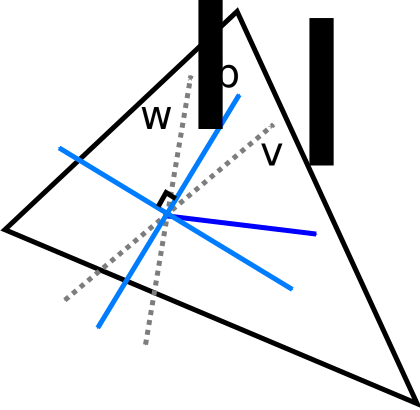
\includegraphics[height=0.8in]{./img/bisector.png}
\caption{$b=\frac{v_i+w_i}{\|v_i+w_i\|}$}
\end{figure}
}{0.55}{
Given a $b$, $v_i,w_i$ can be get by solving conjugate condition, so the problem is how to get $b$.

Options:
\begin{itemize}
\item 4-sys field generation ``Mixed-integer'' (slow but less singularity)
\item propagate from user direction constraint faces.(fast and acceptable field)
\end{itemize}
}
\end{frame}

\begin{frame}{Singularity Editing}
\TwoColumns{0.3}{
\begin{figure}[!htb]
\includegraphics[height=1.0in]{./img/singularity-edit1.png}\\
\vspace{0.3in}
\includegraphics[height=1.0in]{./img/singularity-edit2.png}
\end{figure}
}{0.6}{
  Note: \textcolor{blue}{Index is defined on its bisection field, recalling it's a 4-sys field.}\smallskip

  Singulari Moving:

  (\text{\tiny{please refer to [Trivial Connection],[Geometry Aware]}})
  \begin{itemize}
  \item Calculate Angle defect on start point $K_i^{corr}$and target point $K_j^{corr}$.
  \item $K_i^{corr}-2\pi I$ and $K_j^{corr}+2\pi I$
  \item Update angle defect on each edge $B_{ij}$ by using method in [Trivial Connection]
  \item encode the angle defect into smooth measurement: $r_{ij}=r_{ij}^0 - B_{ij}$
  \end{itemize}
}
\end{frame}

\section{Planar Mesh Generation}
\begin{frame}{Mesh Generation}
\begin{itemize}
\item Global Parameterization(\text{\small{Please refer to [Mixed-integer]}})
  Improvement:
  \[E=\sum area(f_i)[(\frac{\nabla s_i}{\textcolor{red}{\|\nabla s_i\|}}v^T)^2 + (\frac{\nabla t_i}{\textcolor{red}{\|\nabla t_i\|}}w^T)^2 ]\]
\begin{figure}[!htb]
\centering
\includegraphics[height=1.2in]{./img/gp.png}
\caption{Left: without normalization, Right: normalization}
\end{figure}

\end{itemize}
\end{frame}

\begin{frame}{Mesh Generation}
\begin{itemize}
\item Planar constraints
\begin{eqnarray*}
E&=&E_{fair} + E_{2nd} + E_{dist}\\
s.t. 2\pi &=& \phi_{ij}^1+\phi_{ij}^2+\phi_{ij}^3+\phi_{ij}^4
\end{eqnarray*}
\TwoColumns{0.3}{
\begin{figure}[!htb]
\centering
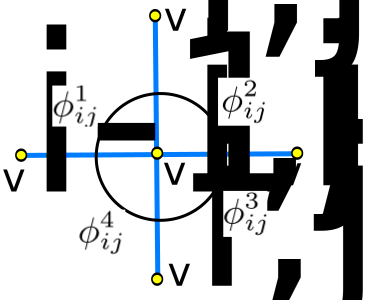
\includegraphics[height=1.0in]{./img/planar.png}
\end{figure}
}{0.55}{
\begin{eqnarray*}
E_{fair} &=& \sum(\|\delta_{i,j,1}\|^2+\|\delta_{i,j,2}\|^2)\\
E_{2nd} &=& \sum(\|\delta_{i,j,1}-\delta_{i,j,1}^0\|^2+\|\delta_{i,j,2}-\delta_{i,j,2}^0\|^2)\\
E_{dist} &=& \sum(\|v_{i,j}-v_{i,j}^0\|^2)\\
\delta_{i,j,1} &=& v_{i-1,j} + v_{i+1,j} - 2v_{i,j}\\
\delta_{i,j,2} &=& v_{i,j+1} + v_{i,j-1} -2 v_{i,j}
\end{eqnarray*}
}
\end{itemize}
\end{frame}

\section{Results}
\begin{frame}{Results}
\begin{figure}[!htb]
\centering
\includegraphics[height=3in]{./img/r2.png}
\end{figure}
\end{frame}

\begin{frame}{Results}
\begin{figure}[!htb]
\centering
\includegraphics[height=3.0in]{./img/r3.png}
\end{figure}
\end{frame}

\begin{frame}{Results}
\begin{figure}[!htb]
\centering
\includegraphics[height=2.0in]{./img/r4.png}
\end{figure}
\end{frame}

\section{Conclusion}
\begin{frame}{Conclusion and Feature work}
\begin{itemize}
\item A novel smooth measurement based on signed-permuation matrix representation for CDF
\item An improvement of global parameterization
\item Lacking explicit singularity control
\item Angle defect is not considered in smooth measurement
\end{itemize}
\end{frame}

\begin{frame}{Q.A}
\end{frame}
\end{document}
